
\documentclass[a4paper,12pt]{article}
\usepackage[utf8]{inputenc}
\usepackage[T1]{fontenc}
\usepackage{amssymb}
\usepackage{amsmath}
\usepackage{mathabx}
\usepackage{graphicx}
\usepackage[all]{xy}
\newtheorem{definicion}{Definición}[subsection]
\newtheorem{teoremas}{Teorema}[subsection]
\newtheorem{ejemplos}{Ejemplo}[subsection]
\newtheorem{observ}{Observación}[subsection]
\newtheorem{prop}{Proposición}[subsection]
\newtheorem{Corolario}{Corolario}[subsection]


\begin{document}

\section{Ejercicio 1}

\subsection{}
\textit{a. Demuestra que un conjunto de medida cero no tiene puntos interiores.}
Primeramente fijaremos algunas definiciones que usaremos para demostrar la proposición.
\begin{definicion}.\\
Sea  $\vec{x_0} \in \mathbb{R}^n$ y $\epsilon > 0$. Se define la bola abierta de $\mathbb{R}^n$
con centro en $\vec{x_0}$ y radio $\epsilon$ por:
\[B(\vec{x_0},\epsilon) = V_{\epsilon}(\vec{x_0}) =
\lbrace \vec{x} \in \mathbb{R}^n |  \Vert \vec{x} - \vec{x_0} \Vert \rbrace\]
\end{definicion}
\begin{definicion}.\\
Sea $A \subseteq \mathbb{R}^n$ y sea $\vec{x_0} \in A$. Entonces $\vec{x_0}$ se llama punto interior de $A$ si existe
$\epsilon > 0$ tal que $B(\vec{x_0},\epsilon) \subseteq A$.
\end{definicion}
\begin{definicion}.\\
Un rectángulo cerrado en $\mathbb{R}^n$ es un conjunto de la forma
\[[a_1 , b_1] \times [a_2,b_2] \times \cdots \times [a_n,b_n]\]
con $a_i,b_i \in \mathbb{R}$, $1 \leq i \leq n$.
Se define el volumen del rectángulo $S = [a_1 , b_1] \times [a_2,b_2] \times \cdots \times [a_n,b_n]$ por:
\[Vol(S) = v(s) = (b_1 - a_1)(b_2 - a_2)\cdots(b_n - a_n) = \prod_{i = 1}^{n}(b_i - a_i)\]
si $a_i \leq b_i$, $\forall 1 \leq i \leq n$ y $Vol(s) = 0$ si $S = \emptyset$.
\end{definicion}
\begin{definicion}.\\
Un conjunto $A \subseteq \mathbb{R}^n$ se dice que tiene medida 0 si dado $\epsilon > 0$, existe un recubrimiento a lo
más numerable $\lbrace U_n \rbrace_{n = 1}^{\infty}$ de $A$ de rectángulos cerrados es decir
\[A \subseteq  \bigcup_{n = 1}^{\infty} U_n\]
con $U_n$ un rectángulo cerrado de $\mathbb{R}^n$, tal que
\[\sum_{i = 1}^{\infty} Vol(U_i) < \epsilon. \]
\end{definicion}
\textbf{Demostración}\\
Sea un $A \subseteq \mathbb{R}^n$ un conjunto de medida 0.Supongamos que A poseé un punto interior $x_0$ por definición
existe un cierto $\epsilon > 0$ tal que $B(x_0,\epsilon) \subseteq A$, ello implica que $B(x_0,\epsilon)$ consta de todos
los puntos $x$ tal que $\Vert x - x_0\Vert < \epsilon$. Ahora dado que A tiene medida 0 existe un recubrimiento de
rectángulos que satisface $A \subseteq  \bigcup_{n = 1}^{\infty} U_n$  tal que
\[\sum_{i = 1}^{\infty} Vol(U_i) < \varepsilon .\]
Para todo $\varepsilon > 0$.Lo que a su vez implica que $B(x_0,\epsilon) \subseteq A \subseteq  \bigcup_{n = 1}^{\infty} U_n$. Puesto que la
desigualdad
\[\sum_{i = 1}^{\infty} Vol(U_i) < \varepsilon .\]
se satisface para cualquier $\varepsilon > 0$. Por lo tanto se tiene que para cualquiera de los subrectángulos
$U_k$ con $k \in \mathbb{N}$,
se satisface que $Vol(U_k) <  \sum_{i = 1}^{\infty} Vol(U_i) < \varepsilon $. Si tomamos un punto $x_0 \in A$ con $\epsilon > \varepsilon $ se hace
evidente que $B(x_0,\epsilon) \not \subset  \bigcup_{n = 1}^{\infty} U_n$ lo cual contradice el hecho de que
$B(x_0,\epsilon) \subseteq A \subseteq  \bigcup_{n = 1}^{\infty} U_n$. Analogamente si tomamos
$\epsilon \leq \varepsilon , \forall \varepsilon > 0$ implica que $B(x_0,\epsilon) \subseteq U_k$ para algun $k \in \mathbb{N}$
o $B(x_0,\epsilon) \subseteq  \bigcup_{n = 1}^{\infty} U_n$, se tiene entonces necesariamente que $\epsilon = 0$ lo cual es una contradicción
puesto que hemos supuesto que $\epsilon > 0$. Por tanto podemos concluir que si A tiene medida cero entonces A no poseé
puntos interiores.$\blacksquare$

\newpage
\subsection{}
\textit{b. Construye un conjunto que tenga medida cero pero que su cerradura sea $\mathbb{R}^n$.\\}
De igual forma establecemos primeramente algunas definiciones que nos ayudaran a demostrar la proposición.
\begin{definicion}.\\
Dado $A \subseteq \mathbb{R}^n$. Un punto $\vec{x_0} \in  \mathbb{R}^n$.Se llama punto de adherencia de A si para todo
$\epsilon > 0, B(x_0,\epsilon) \cap A \not = \emptyset$.\\
El conjunto
\[\overline{A} = \lbrace \vec{x} \in \mathbb{R}^n | \vec{x} \text{ es un punto de adherencia de A} \rbrace\]
recibe el nombre de cerradura de $A$.
\end{definicion}
\textbf{Demostración}\\
Sabemos que un conjunto que tiene medida por el ejercicio no contiene puntos interiores por lo que podemos proponer un
conjunto que tenga medida 0 en $\mathbb{R}$ y cuya cerradura sea precisamente $\mathbb{R}$. Tomando en consideracion lo
anteriormente mencionado sea $A = \mathbb{Q}$, con $\mathbb{Q}$ el conjunto de números racionales procederemos a demostrar
que $\mathbb{Q}$ tiene medida cero en $\mathbb{R}$ para ello consideremos la colección de todos los números racionales De
la forma $p/q$ con $p,q \in \mathbb{Z}$ y con la condición de que $p$ y $q$ sean primos relativos. Sea dicho conjunto
$A = \lbrace r_n\rbrace_{n = 1}^\infty$ y definamos los intervalos
\[I_n = (r_n- \frac{\epsilon}{2^n} , r_n +\frac{\epsilon}{2^n} )\]
Si consideramos la unión de los infinitos intervalos, se cumple que
\[ A \subseteq \bigcup_{n = 1}^\infty I_n \]
Ahora puesto que $Vol(U_k) = \frac{\epsilon}{2^{k-1}}, \forall k \in \mathbb{N}$, se tiene que
\[\sum_{k = 1}^{\infty} \frac{\epsilon}{2^{k-1}} \leq \epsilon \]
la serie anterior converge para cualquier $\epsilon$ que escojamos y preserva la desigualdad, ahora puesto que podemos hacer
$\epsilon$ tan pequeño como queramos se tiene necesariamente que el conjunto $A$ tiene medida cero en $\mathbb{R}$.
Es decir el conjunto $\mathbb{Q} \subset \mathbb{R}$ es de medida cero.
Ahora puesto que $\mathbb{Q}$, es de medida cero y se tiene que la cerradura $\overline{\mathbb{Q}}$ es precisamente
$\mathbb{R}$, tomemos el conjunto
\[\mathbb{Q}^n = \mathbb{Q} \times \mathbb{Q} \times \cdots  \times \mathbb{Q} \]
formado al realizar el producto cartesiano de $\mathbb{Q}$ con sigo mismo n veces. Entoces se hace evidente que
$\mathbb{Q}^n \subset \mathbb{R}^n$ es de medida cero, esto se sigue del hecho de que podemos verificar esto siguiendo los pasos
anteriormente descritos,de que $\mathbb{Q}$ es de medida cero considerando unicamente rectángulos en $\mathbb{R}^n$.
Con ello obtenemos que $\mathbb{Q}^n$ es de medida cero y su cerradura $\overline{\mathbb{Q}}^n$ es $\mathbb{R}^n$.$\blacksquare$

\section{Ejercicio 2}

\textit{Construye una función acotada $f : I \rightarrow \mathbb{R}$ que sea igual a cero en casi todo punto del intervalo
I y que no sea Riemann integrable.}

\begin{definicion} (Riemann-integrabilidad).\\
Una función f definida en [a, b] es Riemann integrable (R-integrable) si existe
un número real $\mathfrak{R} $ tal que para cualquier $\epsilon > 0, \ \exists \delta > 0$, tal que $\forall \mathcal{P}$
partición de [a, b] con $\Vert \mathcal{P} \Vert < \delta$ y toda elección $\xi$ se tiene
\[\vert \mathcal{R}(f,\mathcal{P},\xi)-\mathfrak{R}\vert < \epsilon\]
En este sentido la función $\mathcal{R}(f,\mathcal{P},\xi)$ esta dada por
\[\mathcal{R}(f,\mathcal{P},\xi) = \sum_{i = 1}^{n} f(\xi_i)\vert x_i - x_{i-1}\vert\]
A esta suma la llamaremos \textbf{Suma de Riemann} de f relativa a la partición
$\mathcal{P} = \lbrace a = x_0 < x_2 < \cdots < x_n = b \rbrace$ de [a, b] y la elección
$\xi = \lbrace \xi_1,\xi_2,\ldots,\xi_n\rbrace$, donde $\xi_i \in [x_{i-1},x_i], 1 \leq i \leq n$.
A este número $\mathfrak{R} $ lo denotaremos mediante el símbolo
\[\int_{a}^{b} f(x) dx = \lim_{\Vert \mathcal{P} \Vert \rightarrow 0} \mathcal{R} (f,\mathcal{P} ,\xi) \]
\end{definicion}

\textbf{Demostración}\\
Sea la función $f : [0,1] \subseteq \mathbb{R} \rightarrow \mathbb{R}$ definida por
\[f(x)=
\begin{cases}
    1 &  x \in \mathbb{Q} \cap [0,1]\\
    0 & x \in [0,1]\diagdown \mathbb{Q}
\end{cases}\]
es claro que la función $f$ es igual a 0 en casi todos los puntos del intervalo $[0,1]$, se demostrara que la función $f$
no es Riemann-integrable.
De acuerdo a lo anteriormente mencionado se tiene que si $f$ es R-integrable entonces debe existir un número real
$\mathfrak{R}$ tal que $\forall \epsilon > 0, \exists \delta >0$ de tal modo que
\[\Vert \mathcal{P} \Vert < \delta \Rightarrow  \vert \mathcal{R} (f,\mathcal{P},\xi) - \mathfrak{R} \vert < \epsilon\]
Para toda partición $\mathcal{P}$ de el intervalo [0,1] y toda elección $\xi$.

\newpage
Sea $\mathcal{P} = \lbrace x_0 = 0 < x_1 < x_2 < \cdots < x_n = 1\rbrace$ una partición de intervalo $[0,1]$ tal que
$\Vert \mathcal{P} \Vert < \delta$, para algún $\delta > 0$ y sea $\xi = \lbrace \xi_1,\xi_2,\ldots,\xi_n\rbrace$ una
elección de tal forma que $\xi_i \in [x_{i-1} , x_i]$. Queda claro entonces que el valor de
$\mathcal{R} (f,\mathcal{P},\xi)$ dependera de la elección $\xi$ que escojamos puesto que independientemente de que
$\Vert \mathcal{P}\Vert \rightarrow 0 $ se tendra que cuando menos el intervalo $[x_{i-1},x_i]$ contendra un número
$a \in \mathbb{Q} \cap [0,1]$ y otro $b \in [0,1]\backslash \mathbb{Q}$, sin importar cuan fina sea la partición $\mathcal{P}$.
Ello implica que en este caso la elección $\xi$ determinara el valor de $\mathcal{R} (f,\mathcal{P},\xi)$ puesto que si
tomamos la elección $\xi_{\mathbb{Q}}$ de tal forma que $\forall \xi_i \in \xi_{\mathbb{Q}}, \xi_i \in  \mathbb{Q} \cap [0,1]$
se tendra que

\[\mathcal{R} (f,\mathcal{P},\xi_{\mathbb{Q}}) = \sum_{i = 1}^{n} f(\xi_i)|x_{i} - x_{i-1}| =  \sum_{i = 1}^{n} 1*|x_{i} - x_{i-1}| = 1 \]
Analogamente si tomamos la elección $\xi_{\mathbb{I}}$ de tal forma que
$\forall \xi_i \in \xi_{\mathbb{I}}, \xi_i \in  [0,1] \backslash \mathbb{Q}$ se tendra que
\[\mathcal{R} (f,\mathcal{P},\xi_{\mathbb{I}}) = \sum_{i = 1}^{n} f(\xi_i)|x_{i} - x_{i-1}| =  \sum_{i = 1}^{n} 0*|x_{i} - x_{i-1}| = 0. \]
Por tanto el resultado de $\mathcal{R} (f,\mathcal{P},\xi)$ dependera de la elección $\xi$  y por tanto de existir un número real
$\mathfrak{R}$ este deberia de cumplir que $\Vert \mathcal{P} \Vert  <\delta \Rightarrow \vert 1 - \mathfrak{R} \vert < \epsilon $
y a su vez $\Vert \mathcal{P} \Vert  <\delta \Rightarrow \vert 0 - \mathfrak{R} \vert < \epsilon $. Esto implica que si $\mathfrak{R}$
existe entonces $\mathfrak{R} $ debe de cumplir
\[\mathfrak{R} \in (-\epsilon+1, \epsilon +1 ) \text{ y } \mathfrak{R} \in (-\epsilon, \epsilon)\]
Por lo tanto dicho número $\mathfrak{R} $ no puede existir puesto que de existir deberia pertenecer a dos entornos distintos
al mismo tiempo. Con ello queda demostrado que la función $f$ no es Riemann-integrable.\\
\begin{center}
    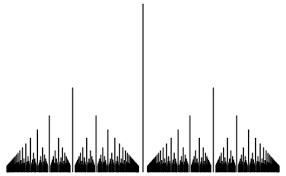
\includegraphics[scale=0.5]{dirichlet.png}
\end{center}


\newpage
\section{Ejercicio 3}
\textit{Demuestra que si f es Riemann integrable sobre un intervalo $I$ y $f (x) = 0$ en casi todos los puntos del intervalo $I$,
entonces}
\[\int_{I} f(x) dx = 0\]
\textbf{Demostración}
Supongamos que $f$ es Riemann-integrable en el intervalo $[a,b]$.Por definición ello implica que $\exists \mathfrak{R} \in \mathbb{R}$
tal que $\forall \mathcal{P} $ partición de $[a,b]$ y $\forall \xi$ elección. Se cumple que $\forall \epsilon > 0, \exists \delta >0$
tal que
\[\vert \mathcal{R}(f,\mathcal{P},\xi) - \mathfrak{R} \vert < \varepsilon.\]

Ahora supongamos que $f(x) = 0$ en casi todo el intervalo $I$ y existe un conjunto a lo más numerable de puntos $\hat{x}$
que satisfacen $f(\hat{x}) \not = 0$. Es evidente entonces que para cualquier elección $\xi = \lbrace \xi_1, \xi_2, \ldots, \xi_n\rbrace$
donde $\xi_i \in [x_i,x_{i+1}]$.
Es decir $\xi_i$ pertenece al subintervalo $[x_i,x_{i+1}]$ de la partición
\[\mathcal{P} = \lbrace a = x_1 < x_2 < \cdots < x_n = b\rbrace\]
y se cumple que cuando menos $\exists \hat{\xi}_1 , \hat{\xi}_2 \in [x_i,x_{i+1}]$ tal que $f(\hat{\xi}_1) = 0$  y
$f(\hat{\xi}_2) \not = 0$.
Por tanto si consideramos la elección $\xi_{\mathcal{O} } = \lbrace \xi_i \in \xi_{\mathcal{O}} : f(\xi_i) = 0\rbrace$
y la elección  $\xi_{\mathcal{Q}} = \lbrace \xi_i \in \xi_{\mathcal{Q}} : f(\xi_i) \not = 0\rbrace$, con $1 \leq i \leq n$.
Si tomamos las sumas de Riemann relativas para las elecciones $\xi_{\mathcal{O}}$,  $\xi_{\mathcal{Q}}$ y la partición $\mathcal{P}$.
Resulta entonces evidente que $\mathcal{R} (f,\mathcal{P},\xi_{\mathcal{O}}) = 0$, ahora si consideramos
$\mathcal{R} (f,\mathcal{P},\xi_{\mathcal{Q}})$ se tiene que puesto que $f$ es R-integrable se satisface que
\[\vert \mathcal{R} (f,\mathcal{P},\xi_{\mathcal{Q}}) - \mathfrak{R} \vert < \varepsilon\]

Ahora sabemos que si hacemos $\Vert \mathcal{P} \Vert \rightarrow 0$, puesto que hemos supuesto que los puntos donde la
función $f$ son  distintos de 0 son un conjunto a lo más numerable implica necesariamente que no importa cuan fina se la
partición se tendra que la elección $\xi$ tendra necesariamente puntos para los cuales $f(\xi_i)$ sea 0. Por tanto se tiene
que cuando menos
\[0 \leq \vert \mathcal{R} (f,\mathcal{P},\xi_{\mathcal{Q}}) - \mathfrak{R} \vert < \varepsilon \]
como podemos hacer $\varepsilon$ tan pequeño como queramos podemos concluir que puesto que $\mathfrak{R}$ existe y cumple
que
\[-\varepsilon - \mathcal{R} (f,\mathcal{P},\xi_{\mathcal{Q}}) <  \mathfrak{R}  < \varepsilon - {\mathcal{R} (f,\mathcal{P},\xi_{\mathcal{Q}})}_{(1)}\]
Puesto que hemos supuesto que la desigualdad anterior se conserva para cualquier partición y elección que tomemos, puesto
que $f$ es R-integrable. Y considerando la elección $\xi_{\mathcal{O}}$ de igual forma satisface la desigualdad podemos
concluir que
\[\int_{I} f(x) dx = 0\]
Es decir si $\mathfrak{R}$ existe la desigualdad $(1)$ se cumple para cualquier suma de Riemann relativa $\mathcal{R} (f,\mathcal{P},\xi)$,
podemos concluir entonces que necesariamente $\mathfrak{R} = 0._\blacksquare$
\newpage
\section{Ejercicio 4}
\textit{Usando la definición de suma de Riemann con ayuda del criterio de Darboux, encuentra}
\[\int_{[0,1] \times [0,1]} (x^2y+x)dxdy\]
Sea $\mathsf{P}$ una partición del rectángulo $[0,1] \times [0,1]$, de tal modo que
$\mathcal{P} = \lbrace \mathcal{P}_1, \mathcal{P}_2 \rbrace$, donde $\mathcal{P}_1$ y $\mathcal{P}_2$ son una partición
del intervalo $[0,1]$

\newpage
\section{Ejercicio 5}
\textit{Sea $f(x,y,z) = z \sin(x+y)$ y considerando el intervalo $[0,\pi]\times[-\pi/2,\pi/2]\times[0,1]$. Usa el teorema
de Fubini para calcular:}
\[\int_{I} f(x,y,z) dxdydz\]


La integral esta dada por

\[\int_{E} f(x,y,z)dxdydz = \int_{0}^{1} \int_{-\pi/2}^{\pi/2} \int_{0}^{\pi} z\sin (x+y) dxdydz\]

\[\int_{0}^{1} \int_{-\pi/2}^{\pi/2} \int_{0}^{\pi} z\sin (x+y) = \int_{0}^{1} \int_{-\pi/2}^{\pi/2} z \left[ \int_{0}^{\pi} \sin (x+y) dx \right] dydz \]

\[ = \int_{0}^{1} \int_{-\pi/2}^{\pi/2} z \left[ -\cos (x+y) \vert_{y}^{y + \pi} \right] dydz = \int_{0}^{1} \int_{-\pi/2}^{\pi/2} z \left[ 2\cos (y)\right] dydz\]
\[ = \int_{0}^{1} 2z\left[\int_{-\pi/2}^{\pi/2}  \cos (y) dy\right] dz =  \int_{0}^{1} 2z\left[\sin(y) \vert_{-\pi/2}^{\pi/2}\right] dz\]
\[ = \int_{0}^{1} 4z dz = 4 \int_{0}^{1} z dz = 4 (\frac{z^2}{2}\vert_{0}^1) = 2 \]

\newpage
\section{Ejercicio 6}
\textit{Usa el teorema de Fubini para mostrar que si una función $f : D \subset \mathbb{R}^2 \rightarrow \mathbb{R}^m$
para algún $m \geq 1$, entonces}
\[\frac{\partial^2 f}{\partial x \partial y} = \frac{\partial^2 f}{\partial y \partial x}.\]

\end{document}
